\section{Thickness and size of the shield}\label{sec:5:shield-size}
The thickness and size of the shield can be estimated by considering a real material. The shield material should have a large electric conductivity $\sigma$ and should therefore behave like an conductor. Even a superconducting shield could be considered.
For a real metal like for example copper, the transmission $T$ of electromagnetic waves is given by \cite{Vandenbosch_2022}
\begin{equation}
  T = \abs{\frac{\vec{E}_\mathrm{after}}{\vec{E}_\mathrm{before}}} = \frac{2}{Z_0 \sigma d}
\end{equation}
where $\sigma$ is the electric conductivity, $Z_0 = 377\si{\Omega}$ the impedance of free space (provided the shield is placed in a vacuum or air) and $d$ the thickness of the shield.
The electric conductivity has a strong dependence on temperature and decreases with $1/T^5$ \footnote{This behavior is only true for temperatures below the Debye temperature. For copper, this limit is around $\Theta_D = 343\si{K}$. In the experiment, the shield is cooled down, so the low-temperature limit of the electric conductivity for metals is very valid \cite{Berman_1952}.} with increasing temperatures \cite[p. 284-286]{Gross_2018}. The electric conductivity for copper at room temperature ($\sigma = 59.6\times 10^6 \si{S/m}$) should therefore be a very valid worst-case approximation. 
Measured data suggest a conductivity of $\sigma(T = 10) \approx 1.5\times 10^{10}\si{S/m}$ \cite{Berman_1952}.

In general should the thickness of the shield be chosen as thin as possible. Otherwise, the distance between the masses has to increase accordingly and the gravitational potential between them gets smaller. This would require longer coherence times till a sufficient amount of entanglement could be measured.
To estimate the thickness of the shield, I am using the condition, that entanglement between the masses should be built up mainly due to gravity. All other possible interactions like Coulomb or Casimir forces, should be suppressed sufficiently by the shield.
To quantify the amount of entanglement built-up over time, I obt for a measure called \emph{entanglement rate}
\begin{equation}\label{eq:5:entanglement-rate}
  \Gamma = \dv{t} E_N(\rho)\Big|_{t=0}
\end{equation} 
where $E_N$ is an appropriate entanglement measure - in this case the logarithmic negativity from \cref{sec:2:entanglement-measures}.
For the gravitational entanglement, this can be calculated by eq. \eqref{eq:2:entanglement-dynamics-parallel} and for the parallel configuration this is given by
\begin{equation}\label{eq:5:entanglement-rate-gravity}
  \Gamma_\mathrm{Gravity} = \frac{G M_A M_B (\Delta x)^2}{16 \hbar L^3 \log 2} .
\end{equation}
The entanglement rate for other interactions should be smaller (and ideally a lot smaller) than the entanglement rate due to gravity.
In the following, this is considered for Coulomb- and Casimir interactions.

\subsection{Shielding Coulomb-Interactions}
The main focus of the shield is to block electromagnetic interactions between the spheres.
Experimentally, it might be beneficial for the spheres to carry a small amount of charge to help with the trapping. !!!CITATIONS!!!
The Coulomb interaction potential energy
\begin{equation}
  V = \frac{1}{4\pi\varepsilon_0} \frac{q_A q_B}{2L}
\end{equation}
between the spheres has the same structure as the gravitational potential and can therefore induce entanglement by the same logic.
Using a shield, this coupling is suppressed by a factor of $T$.
The entanglement rate $\Gamma_\mathrm{Coulomb}$ is therefore easily calculable in a similar form as eq. \eqref{eq:5:entanglement-rate-gravity} to
\begin{equation}\label{eq:5:entanglement-rate-coulomb}
  \Gamma_\mathrm{Coulomb} = \frac{T \abs{q_A q_B} (\Delta x)^2}{64 \pi \varepsilon_0 \hbar L^3 \log 2}
\end{equation}
Requiring that $\Gamma_\mathrm{Gravity} > \Gamma_\mathrm{Coulomb}$, this inequality yields a maximum transmission and thus a minimum thickness of
\begin{align}\label{eq:5:coulomb-gravity-condition}
  T \frac{\abs{q_A q_B}}{4 \pi \varepsilon_0} \, &< \, G M_A M_B \\
  \Longleftrightarrow \quad\quad\quad\quad d \, &> \, \frac{1}{2 \pi \varepsilon_0 Z_0 \sigma G} \frac{\abs{q_A q_B}}{M_A M_B} = \frac{9}{32}\frac{1}{Z_0 \sigma} \frac{1}{\pi^3 \varepsilon_0 G \rho^2} \frac{e^2}{R^6}
\end{align}
where in the last step $M_A = M_B$ and $q_A = q_B = e$ has been assumed.
The shield thickness heavily depends on the radius of the spheres where small and light masses make the shield unworkably thick.
A silica sphere with a radius of $R=10^{-5}\si{m}$ would require a shield around the thickness of $10\si{nm}$ at $4\si{K}$ up to $2.5\si{\mu m}$ at room temperature.
A realistic thickness for the shield at low temperatures could therefore be $d=100\si{nm}$.

Electric fields however can still propagate around a Faraday shield of finite size and induce entanglement. It is however possible, to estimate the required radius $r_s$ of the shield to block a specific amount $\eta$ of the electric field.
The resulting radius corresponding to $\eta$ is derived in appendix \ref{apx:blocking-of-the-shield} and the result is shown in \cref{fig:5:shield-radius}.
\begin{figure}[!ht]
  \centering
  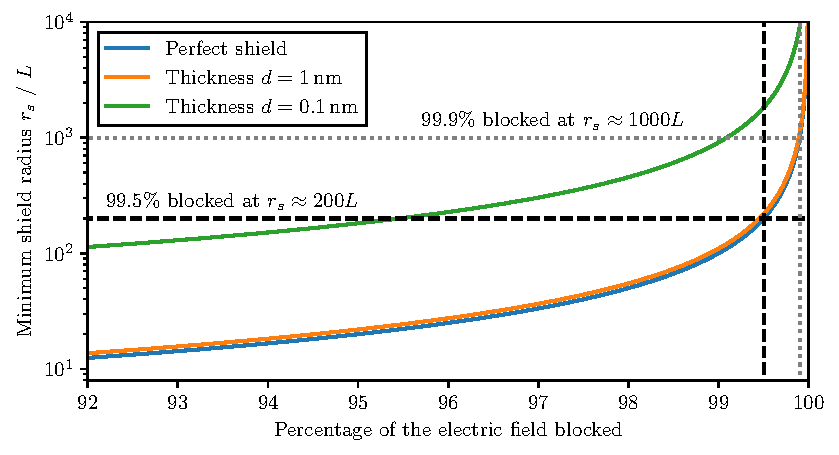
\includegraphics[width=\textwidth]{./../figures/others/shield-radius.pdf}
  \caption{Radius of the shield depending on the shield effectiveness $\eta$. Additionally a real shield with different thicknesses $d$ at room temperature is considered. For a shielding between $99.5...99.9\%$ ($\eta = 0.995...0.999$), a radius of at least $r_s =200...1000L$ should be used. For a sphere-plate distance of $L=2 \times 10^{-5}\si{m}$, the shield radius should be in the order of millimeters and centimeters.}
  \label{fig:5:shield-radius}
\end{figure}
The transmission $T$ should be replaced by a modified transmission $\tilde{T} = T\eta + (1-\eta)$ where the shield effectiveness $\eta$ depends on $r_s$. 
Now, the condition eq. \eqref{eq:5:coulomb-gravity-condition} introduces a limit for the minimum effectiveness and thus a limit on the minimum radius of
\begin{equation}
  \eta_\mathrm{min} = 1 - \frac{4\pi \varepsilon_0 G M_A M_B}{\abs{q_1 q_2}} .
\end{equation}
Thus using the setup with the parameters from earlier, a minimum effectiveness of $\eta_\mathrm{min} \gtrsim 0.99997$ and thus a radius of $\gtrsim 66\si{cm}$ is required.
This shield is too large for all practical purposes and it might be beneficial to choose slightly heavier masses to reduce the shield size to the orders of $\sim 1\si{cm}$. This would require both spheres to have approximately double the radius than before.
Using neutral masses without any charge would is also beneficial and the shield size could be reduced to only the size of the spheres themselves, however it might be an engineering challenge, to trap and levitate uncharged massive particles.





\subsection{Shielding Casimir-Interactions}
Similarly to Coulomb interactions, it is possible to to estimate the required thickness of the shield necessary to sufficiently suppress Casimir interactions. Between two spheres with radius $R$ and separation $2L$, the Casimir potential reads \cite{Emig_2007}
\begin{equation}
  V = -\frac{23 \hbar c}{4\pi \cdot 128 L^7} \left( \frac{\varepsilon_r - 1}{\varepsilon_r + 2} \right)^2 R^6 .
\end{equation}
The entanglement rate can be obtained similarly as before by expanding the casimir potential between the spheres in small $\Delta x$ and computing the logarithmic negativity as before:
\begin{equation}
  \Gamma_\mathrm{Casimir} = T^2 \frac{161}{4096} \frac{c R^6 (\Delta x)^2}{\pi L^9 \log 2}\left( \frac{\varepsilon_r - 1}{\varepsilon_r + 2}\right)^2 .
\end{equation}
The dependence on $T^2$ is only a systematic guess but should be sufficient for a basic estimation. Casimir and van der Waals forces are second order effects in the dipole-dipole interaction \cite{Bordag_2001}.
Demanding again, that the entanglement due to gravity should be mediated faster than due to Casimir interactions $\Gamma_\mathrm{Gravity} > \Gamma_\mathrm{Casimir}$, one arrives at the expression
\begin{align}
  T^2 \frac{161 c R^6}{256 \pi L^6} \left( \frac{\varepsilon_r - 1}{\varepsilon_r + 2}\right)^2 \, &< \, \frac{G M_A M_B}{\hbar} \\
  \Longleftrightarrow \quad\quad\quad d^2 \, &> \, \frac{4 \cdot 161 c \hbar R^6}{256 Z_0^2 \sigma^2 \pi L^6 G M_A M_B} \left( \frac{\varepsilon_r - 1}{\varepsilon_r + 2}\right)^2 \\
  \Longleftrightarrow \quad\quad\quad\  d \, &> \, \sqrt{\frac{1449}{4096} \frac{c \hbar}{G \pi^3}} \frac{2}{Z_0 \sigma \rho L^3} \frac{\varepsilon_r - 1}{\varepsilon_r + 2}
\end{align}
where again in the last step I assume $M_A = M_B$. For large separations, the shield thickness can go arbitrary low because of the weakness of the casimir interactions at larger distances. Between two silica spheres separated in the order of magnitude as the radius ($L = 2\times 10^{-5}\si{m}$), the required minimum thickness is between $4\times 10^{-11}\si{m}$ at $4\si{K}$ and $10 \si{nm}$ at room temperature.
Either way, it is much thinner than a Faraday shield required to shield electrostatic Coulomb interactions. The effect of $\varepsilon_r$ was neglected in these numbers. The minimum thickness only changes by a factor between $0...1$ due to dielectric materials.
In fact, these thicknesses are much thinner than recommended, because the shield loses rigidity.
It turns out that the vibrational frequency depends linearly on the thickness and thus more vibrations are possible. A more detailed discussion of this matter is given in the next section.


\subsection{Gravitational effects of the shield}
For simplicity, in the following estimations of the attractive gravitational force between an infinitely large plate with thickness $d$ and a sphere positioned a distance $L$ in front of the plate is calculated. This should slightly overestimate the actual force due to a finite plate \footnote{In fact, using a finite shield with radius $r_s = 0.01\si{m}$, the total force decreases only by $0.2\%$ compared to an infinitely sized one.}.
The gravitational force between the sphere and a infinitesimal mass segment $\dd m = r \rho d \dd r\dd \varphi$ of the plate with density $\rho$ at a distance $r$ from the center is given by
\begin{equation}
  \dd \vec{F} = \frac{G M \dd m}{\ell^2} \boldsymbol{\hat{\ell}} 
  \quad \Rightarrow \quad
  \dd F_z = \frac{G M r \rho d}{\ell^2} \dd r \dd \varphi \cos \theta,
\end{equation}
where $\ell^2 = r^2 + L^2$ denotes the distance between the sphere and the mass segment and $\theta = \arccos L/\ell$ is the angle between them. % (see \cref{fig:5:plate-gravity}).
The total force between the sphere and the infinite plate is therefore given by
\begin{equation}
  F_z = GM \rho d L \int_{0}^{\infty} \dd r \int_{0}^{2\pi} \dd \varphi \, \frac{r}{(r^2 + L^2)^{3/2}} = 2 \pi G M \rho d .
\end{equation}
% \begin{equation}
%   F_z = GM \rho d L \int_{0}^{r_s} \dd r \int_{0}^{2\pi} \dd \varphi \, \frac{r}{(r^2 + L^2)^{3/2}} = 2 \pi G M \rho d \left[1 - \frac{L}{\sqrt{L^2 + r_s^2}}\right].
% \end{equation}
This result is independent of the distance $L$ and a numerical value for a copper shield ($\rho = 8960\si{kg/m^3}$) with thickness of $d = 100\si{nm}$ and the silica sphere already used in \cref{cha:first-look} is given by $F \approx 4.2 \times 10^{-24}\si{N}$.
Compared with the attractive force between two silica spheres separated by a distance of $2L = 4\times 10^{-5}\si{m}$, the force due to the plates is smaller by a factor of of $\approx 0.8$.
%% F = 5.132 \times 10^{-24} \si{N}
Both forces are therefore comparable and the thickness of the shield should be chosen as thin as possible to not influence the gravitational sensing of the masses. 
If the shield is not perfectly placed in the center between the two masses or if the shield is uneven due to e.g. thermal vibrations, these gravitational effects might be able to destroy entanglement by inducing non-global phases to the cat-states.